%%%%%%%%%%%%%%%%%%%%%%%%%%%%%%%%%%%%%%%%%%%%%%%%%%%%%%%%%%%%%%%%%%%%%%%%%%%%%%%%
%2345678901234567890123456789012345678901234567890123456789012345678901234567890
%        1         2         3         4         5         6         7         8

\documentclass[letterpaper, 10 pt, conference]{ieeeconf}  % Comment this line out if you need a4paper

%\documentclass[a4paper, 10pt, conference]{ieeeconf}      % Use this line for a4 paper

\IEEEoverridecommandlockouts                              % This command is only needed if 
                                                          % you want to use the \thanks command

\overrideIEEEmargins                                      % Needed to meet printer requirements.

% See the \addtolength command later in the file to balance the column lengths
% on the last page of the document

% The following packages can be found on http:\\www.ctan.org
\usepackage{graphicx} % for pdf, bitmapped graphics files
%\usepackage{epsfig} % for postscript graphics files
%\usepackage{mathptmx} % assumes new font selection scheme installed
%\usepackage{times} % assumes new font selection scheme installed
\usepackage{amsmath} % assumes amsmath package installed
\usepackage{amssymb}  % assumes amsmath package installed
\usepackage{multicol}

\title{\LARGE \bf
Final Report: Analysis of Security In a Modern Processor
}


\author{Justin Cox and Tyler Travis
\\ \small{Department of Electrical and Computer Engineering}
\\ \small{Utah State University}
\\ \small{Logan, Utah 84322}
\\ \small{email: justin.n.cox@gmail.com, tyler.travis@aggiemail.usu.edu}
}

\usepackage{listings}
\usepackage{color}

\definecolor{dkgreen}{rgb}{0,0.6,0}
\definecolor{gray}{rgb}{0.5,0.5,0.5}
\definecolor{mauve}{rgb}{0.58,0,0.82}

\lstset{frame=none,
  language=C,
  aboveskip=3mm,
  belowskip=3mm,
  showstringspaces=false,
  columns=flexible,
  basicstyle={\small\ttfamily},
  numbers=none,
  numberstyle=\tiny\color{gray},
  keywordstyle=\color{blue},
  commentstyle=\color{dkgreen},
  stringstyle=\color{mauve},
  breaklines=true,
  breakatwhitespace=true,
  tabsize=3
}


\begin{document}



\maketitle
\thispagestyle{empty}
\pagestyle{empty}


%%%%%%%%%%%%%%%%%%%%%%%%%%%%%%%%%%%%%%%%%%%%%%%%%%%%%%%%%%%%%%%%%%%%%%%%%%%%%%%%
\begin{abstract}

Hardware security is an ever increasing area of study since exploits have been found on computer systems. It has been found that attackers are able to look at the memory of a system to see what is being processed. This paper proposes adding an extra level of security between the memory and the pipeline. This layer of security would encrypt data headed to memory and decrypt the data headed to the pipeline making the data held in memory incomprehensible to an attacker. To make the added cryptographic system more secure, research will be done on the benefits of utilizing a Physically Unclonable Function (PUF). Further analysis will be done on how this will affect the processor's performance.

\emph{Index Terms}---encryption, decryption, security, pipeline, PUF.

\end{abstract}

%%%%%%%%%%%%%%%%%%%%%%%%%%%%%%%%%%%%%%%%%%%%%%%%%%%%%%%%%%%%%%%%%%%%%%%%%%%%%%%%
\section{INTRODUCTION}

Over the years, there have been many advancements made to computer systems and architecture. These advancements have been primarily focused on improving performance and power consumption. As a result, the security of these architectures has been neglected. Malicious attacks on computer systems are becoming more common and as a result, there is greater need for more secure systems.

The optimal solution to this problem is to completely redevelop the architectures with security as a top priority. However this option is not very practical as it would be far too expensive to replace the current processors and there is a need to support legacy machines. Therefore, we propose to create security modules that can be added to current processor architecture.

This paper shows the authors' process of developing a DES cryptography module designed to be inserted into the gem5 simulation software.  The paper also shows how a PUF can be used to increase the security of the DES module.  The results of the architecture's performance with the added security module will be simulated and the results will be given. 

%%%%%%%%%%%%%%%%%%%%%%%%%%%%%%%%%%%%%%%%%%%%%%%%%%%%%%%%%%%%%%%%%%%%%%%%%%%%%%%%
\section{BACKGROUND}

Computer security is becoming more important as more systems and devices are being compromised.  In particular, there has been an increased number of attacks focused on stealing information stored in memory on computers and servers.  This information can be encrypted when not in use, but currently there are very few solutions that allow the computer architecture to work with the encrypted data.  As a result, when the architecture is running, the data stored in memory is vulnerable to attackers.

Previous research has been done on the development and implementation of secure processors [1].  Similar to the previous research done, this paper will focus on data encryption and decryption and the toll it takes on processor performance.  The objective is to provide as much security as possible without reducing the performance heavily.

%%%%%%%%%%%%%%%%%%%%%%%%%%%%%%%%%%%%%%%%%%%%%%%%%%%%%%%%%%%%%%%%%%%%%%%%%%%%%%%%
\section{TECHNIQUE}

The following subsections will describe the techniques used to supply current computer architecture with more data security. The first subsection will describe how the data will be protected by cryptography. The last section will describe how the cyptograhic modules will be improved using a PUF.

\subsection{Encryption and Decryption of Data}

The memory can be modified by an attacker and as a result the attacker is able to change the execution flow of a program.  Since the data is not encrypted, the attacker is also able to steal important information that may be contained in memory. Therefore to prevent the attacker from knowing where to modify or read the data, it is important for the CPU to encrpyt data being stored into memory. Initially, we will encrypt memory that is stored in registers, cache, RAM, and virtual memory [1]. If the performance decreases significantly, encryption will be excluded from the registers and/or cache. Assuming the pipeline is trusted, data being pushed into the pipeline will be decrypted.

These encryption and decryption modules will be built and inserted into the gem5 source code.

\subsection{Data Encryption Standard (DES)}

The type of encryption used for the module will be DES.  Although DES is not the current encryption standard and is not as secure as the Advanced Encryption Standard AES, DES will allow better processor performance while still making the data more secure.

A brief overview of DES will be given so that the reader has a better understanding of how encryption could take a toll on processor performance.  If the reader would like an in-depth understanding of DES, it is recommended that the reader look to other sources [2].

The DES algorithm takes a 64-bit plain text input.  It is then run through an initial permutation that outputs 56-bits when are then split into two halves.  The data goes through sixteen rounds that each have a sub-key that is generated for each round based on the original 64-bit DES key.  After the sixteenth round, the output is run through a finial permutation and the algorithm outputs a 64-bit encrypted cipher text.  The rounds are illustrated in Figure 1.

\begin{figure}[thpb]
	\centering
	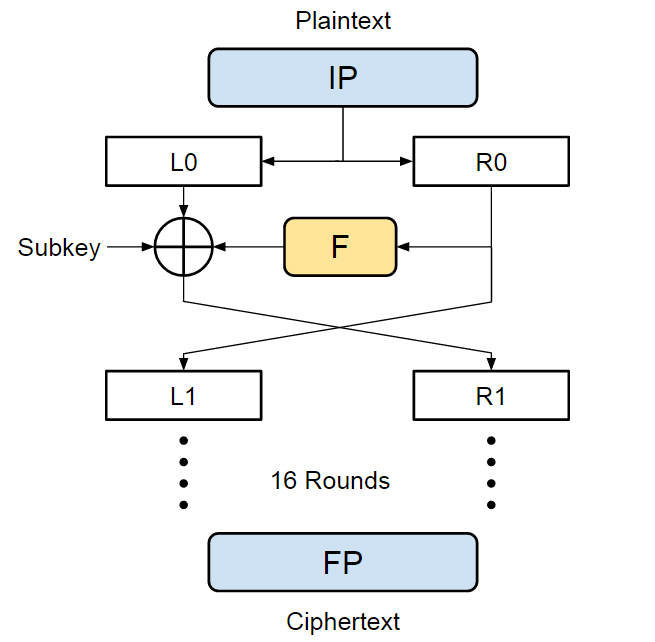
\includegraphics[scale=.50]{DesRounds}
    \caption{An illustration of the sixteen round DES algorithm.}
\end{figure}

During each round, the left 32-bit halve is XORed with the sub key corresponding to the current round as well as the output of the F-function.  The inside functionality of the F-function is illustrated in Figure 2. The output of the XOR is used as the next round's right halve and the next round's left halve is the previous round's right halve.

\begin{figure}[thpb]
	\centering
	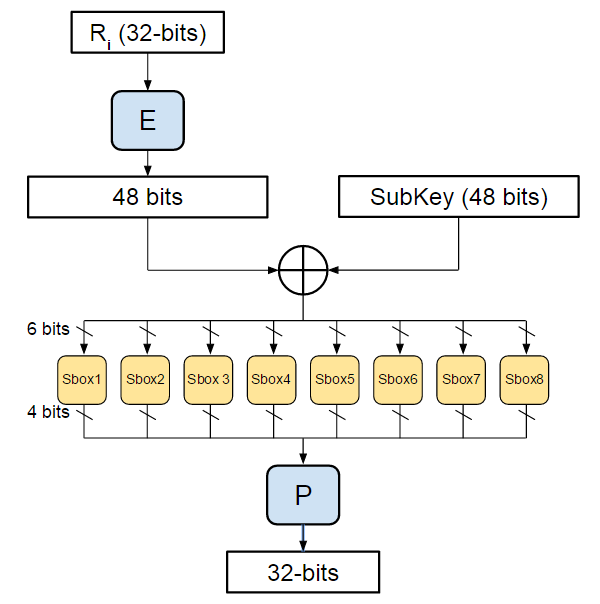
\includegraphics[scale=.50]{Ffunction}
    \caption{An illustration of the F-function}
\end{figure}


\subsection{Physically Unclonable Function (PUF)}

A Physical Unclonable Function (PUF) is a physical entity used to produce information that can only be reproduced using the same physical device.  Since physical imperfections and deviations are normal in the manufacturing and design process of circuits and devices, each different device of the same family should have different physical characteristics that only pertain to said device.  These imperfections, whether they be voltage levels, temperature, or delay times, can be used to produce information.

PUFs are especially effective when used in security.  Since PUFs are generally difficult to model, the only way an attacker could recover the information generated by the PUF is to steal the actual physical device.  Even then, if the attacker where to inspect the PUF they would risk changing the physical characteristics of the device and the PUF's output may change.

There are many different types of PUFs such as Optical PUFs, Delay PUFs, and SRAM PUFs [3].

\subsection{Secret Key Generation Using a PUF}

A PUF is used to generate secrets extracted from a physical device due to manufacturing differences. This uniqueness can be used for secure key generation for encryption/decryption [4].

One of the difficulties of using a PUF for secret key generation is the value of \emph{$\mu$intra}.  The measurement \emph{$\mu$intra} is used to determine how much the output response changes of a certain PUF when given the same input challenge.  Ideally, a PUF should generate the same response when given the same challenge.  Two different PUFs should also generate a different response when given the same challenge.  This measurement is referred to as \emph{$\mu$inter}.  A good PUF should have a \emph{$\mu$inter} close to $50\%$ and a \emph{$\mu$intra} close to $0\%$.

The reason \emph{$\mu$intra} is important is because in a encryption/decryption algorithm, even the slightest change to the secret key will change the cypher-text dramatically.  This means that in order to use a PUF for secret key generation, the PUF's challenge-response pairs need to be consistent.  Since this is almost impossible to do using a PUF, Error Correcting Code (ECC) may be used to fix the response output.  A flow chart of this design is shown in Figure 3.

\begin{figure}[thpb]
	\centering
	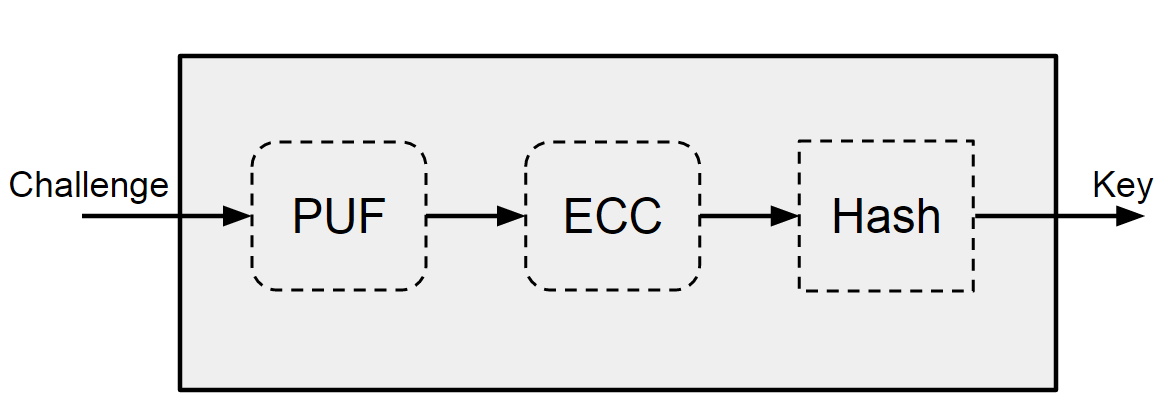
\includegraphics[scale=.25]{keyGen}
   \caption{Flow chart of the secret key generation process.}
\end{figure}

To fix this, majority voting may be used to determine what bits of the response output typically change given the same challenge input.  This process is explained in detail in [5], but a brief overview of the process will be given.  A chosen challenge message is sent through the PUF multiple times.  It is then determined which bits have a tendency to change.  These bits are thrown out and the new challenge message is sent in the ECC.  The ECC encoding process will return parity bits associated with the certain challenge message.  During normal operation, these parity bits can be used to fix the response output for a given challenge.  This process makes sure that the secret key remains the same for a given challenge.

As shown in Figure 3, it is also a good idea to hash the output from the ECC to inhibit the attacker from knowing the response message.  The design can be made even more secure by adding a hash function to the challenge input as well.  

\subsection{Problems to Consider with PUF Implementation}

Although secret key generation using a PUF is a good way to increase the security of the DES algorithm, there are many challenges that are introduced to the proposed security module.  One of the problems to consider is how much the PUF changes after a reboot of the system.  Since the data on the system has been encrypted using the PUF on a previous reboot, the same challenge/response pair needs to be used to decrypt the information.  If the PUF changes due to reboot variations, the CPU will no longer be able to use the stored data.

Another problem that may be introduced is the ability to keep track of the different challenge/response pairs used in the security module.  There are two options available.  One option is to only use one challenge/response pair.  Although this facilitates keeping track of the challenge/response pair, it makes the security module less secure.  If an attacker was able to guess or intercept the response, the system would be compromised.  The other option is to change the challenge/response pair every now and then.  While increasing security, it creates the necessity to keep track of which data corresponds to which challenge/response pair.  This record keeping could become very complex as some of the encrypted data on the system could not be used for a very long time.

This paper will not go over the solutions to these problems, but research has been done to overcome these problems [6].  

\section{METHODOLOGY}

\subsection{Benchmarking and Performance}

The simulator that this project is using is gem5. The security module will be added into the source code for the o3 CPU. Extensive research had to be done in order to determine the right sections of code where the encrypt and decrypt modules need to be added.  The o3 CPU in gem5 can use the SPEC2k6 benchmarks.  A group of these benchmarks will be used to measure the performance of the o3 CPU.  The benchmarks will first be ran without any modifications to the gem5 source code.  In order to have more robust results, the benchmarks will be ran using two different pipeline widths of two and eight.  The same procedure will be repeated but this time the benchmarks will be ran with the security modules inserted into the gem5 source code. The performance will be compared between the two groups of benchmarks.  The benchmarks chosen to be evaluated and compared on performance are:

\begin{multicols}{2}
\begin{itemize}
\item bzip2
\item gcc
\item bwaves
\item mcf
\item gobmk
\item hmmer
\item GemsFDTD
\item libquantum
\item tonto
\item omnetpp
\end{itemize}
\end{multicols}

Since the security module only affects the memory operations in the CPU, the benchmarks that have many store and load instructions will see the greatest performance hit.

\subsection{DES Security Module Code}

The DES encryption and decryption code was written in C++.  In order to work with the gem5 source code, the syntax rules and file naming nomenclature used in gem5 were used.  The code is organized in a header file named \emph{des.hh} and a source code file named \emph{des.cc}.  The code is comprised of many sub-functions, but the two functions that will be called in the gem5 source code are the \emph{encrypt()} function and the \emph{decrypt()} function.  The function prototypes look like the following:

\begin{lstlisting}
void encrypt(uint8_t *plain_text, uint16_t plain_text_size, uint8_t *cipher_text, uint8_t key[8]);

void decrypt(uint8_t *plain_text, uint8_t *cipher_text, uint8_t key[8]);
\end{lstlisting}

The functions take a 64-bit plaintext array and a 64-bit key array.  Since DES works with plaintext of size 64-bits, it needs to be ensured that the data that is encrypted and decrypted in gem5 is a multiple of 64-bits.

\subsection{Modifications Made to gem5 Source Code}

The authors began looking into the source code that handles load and store instructions.  The encryption function needs to be called every time a store instruction is executed.  The decryption function needs to be called every time a load instruction is executed.

After going up the hierarchy in the code, the authors were able to determine that gem5 uses a packet class to be allow the CPU to communicate with the memory.  These packets will be used to encrypt and decrypt the data.  Figure 4 illustrates how the packets are used to encrypt the memory system.  It should be noted that the registers are not encrypted.  This presents a potential security flaw in the system because if an attacker gains control of program flow, he may be able to obtain important information stored in registers.  In a future revision of this project, the authors would like to encrypt the registers as well.

\begin{figure}[thpb]
	\centering
	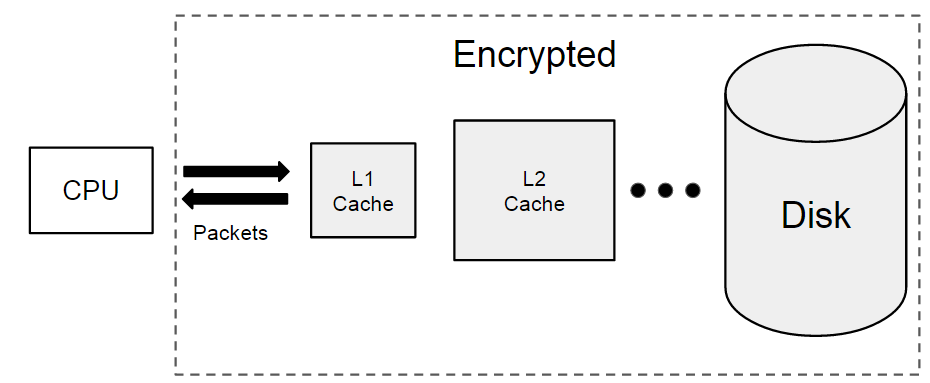
\includegraphics[scale=.35]{gem5}
   \caption{Illustration to show what is being encrypted with the added security module.}
\end{figure}

The gem5 source files that received modifications are \emph{lsq\_unit.hh} and \emph{lsq\_unit\_impl.hh}.
  

\subsection{Environment Used to Run Simulation}

The simulations will be carried out using gem5 on a Linux machine.  The benchmarks will be ran starting at a certain checkpoint to ensure that the performance measurements only include the benchmark and not additional overhead from CPU startup.  The benchmarks will each be ran  until the 100 millionth instruction is reached.

Since each benchmark simulation has the potential to require more than an hour to complete, the simulation process is very time consuming.  To overcome this, the benchmarks will be ran on a cluster of Linux machines using condor.  The results of each benchmark simulation are stored in a text file and the text files will be compared to generate the results.   

\section{RESULTS}



\section{FUTURE WORK}

As mentioned in the subsection C of section IV, the CPU registers are currently not being protected with encryption.  Given more time, the authors would like to upgrade the security module to include the register files.  This would be an improvement with regards to security, but it will also affect the performance.  If the encryption and decryption regarding the registers requires too much of a performance hit, it may end up not having an overall improvement.  The  effects of this added security would need to be tested and simulated in a future work.

Another improvement that can be done to the current security module is to optimize the DES source code.  The code was written as a proof of concept, thus it is not optimized to run efficiently.  Based on the results of this paper, the CPU has a performance decrease when the security module is introduced.  In order to mitigate the performance decrease, the code needs to be optimized as much as possible.

\section{CONCLUSION}

\addtolength{\textheight}{-12cm}   % This command serves to balance the column lengths
                                  % on the last page of the document manually. It shortens
                                  % the textheight of the last page by a suitable amount.
                                  % This command does not take effect until the next page
                                  % so it should come on the page before the last. Make
                                  % sure that you do not shorten the textheight too much.

%%%%%%%%%%%%%%%%%%%%%%%%%%%%%%%%%%%%%%%%%%%%%%%%%%%%%%%%%%%%%%%%%%%%%%%%%%%%%%%%



%%%%%%%%%%%%%%%%%%%%%%%%%%%%%%%%%%%%%%%%%%%%%%%%%%%%%%%%%%%%%%%%%%%%%%%%%%%%%%%%



%%%%%%%%%%%%%%%%%%%%%%%%%%%%%%%%%%%%%%%%%%%%%%%%%%%%%%%%%%%%%%%%%%%%%%%%%%%%%%%%

%\section*{ACKNOWLEDGMENT}

%The author would like to thank his instructor Dr. Rajnikant Sharma %for his help in understanding control concepts.




%%%%%%%%%%%%%%%%%%%%%%%%%%%%%%%%%%%%%%%%%%%%%%%%%%%%%%%%%%%%%%%%%%%%%%%%%%%%%%%%




\begin{thebibliography}{99}

\bibitem{c1} G. Edward Suh, C. W. O'Donnel, I. Sachdev, and S Devadas. Design and Implementation of the AEGIS Single-Chip Secure Processor Using Physical Random Functions. \emph{Proceedings of the 32nd annual international symposium on Computer Architecture}, 2005.
\bibitem{c2} M. Deutschman, "Cryptographic Applications with Physically Unclonable Functions," M.S. Thesis, Inst. Mathematics, Alpen-Adria-Universit\"{a}t Klagenfurt, Klagenfurt, Austria, 2010.
 
\end{thebibliography}


\end{document}
